\chapter{Extending Greedy Recovery to Multiple Communities} \label{chapter 5}
After a thorough exploration of the two-community scenario, we now turn our attention to assessing the performance of the greedy recovery algorithm in the context of five-community case.
\section{Experimental Results for k = 5 in Hard Regime}
\begin{figure}[ht]
    \centering
    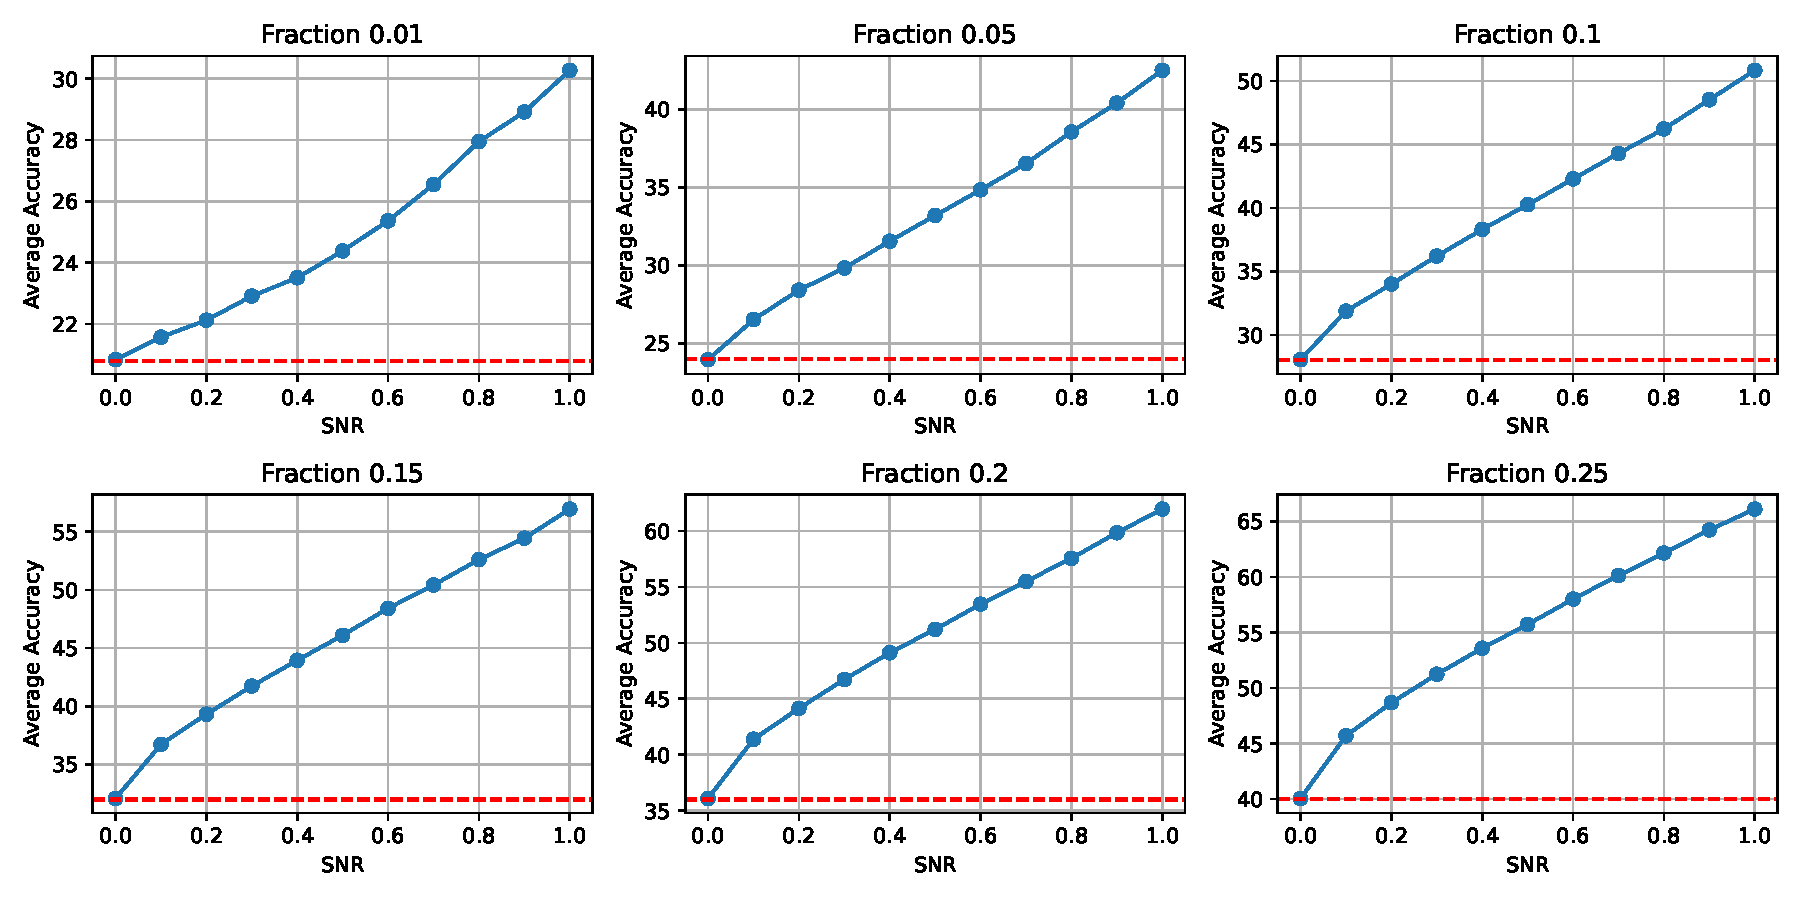
\includegraphics[width=1\linewidth]{Figures/multi_groups_sparse(modified)_1.pdf}
    \caption[Accuracy of Greedy Recovery Algorithm in Sparse Graph with $k=5$]{As in previous figures, the blue line and red dashed lines represent the accuracy of the greedy recovery algorithm and random guess, respectively. The experiment results are averaged over 10 instances with $n=10^5$ and $c=3.$}
    \label{fig: multi_groups}
\end{figure}
From Figure \ref{fig: multi_groups}, we can observe that our greedy algorithm noticeably outperforms random guessing, even for the case of $k=5$ communities.\\
However, our Claim \ref{claim2} does not guarantee the effectiveness of our greedy recovery algorithm for sparse graphs when $k=5$, as it requires $|\Re_v| > 12$ for the claim to be valid under the five-community case.